\documentclass[12pt]{article}
\usepackage[russian]{babel}
\usepackage[left=2.5cm, right=2.1cm, top=2cm, bottom=2cm]{geometry}
\linespread{1.3}
\usepackage{indentfirst}
\usepackage{secdot}
\usepackage{amsmath}
\usepackage{graphicx}
\usepackage{multirow}

\title{Работа 1.2.5 \\ Исследование прецессии уравновешенного гироскопа}

\date{}

\author{Шульгин Константин}

\begin{document}

\maketitle

%######################################################################################
\section*{Цель работы}
Исследовать вынужденную прецессию гироскопа; установить зависимость скорости вынужденной прецессии гироскопа от величины момента сил, действующих на ось гироскопа; определить скорость вращения ротора гироскопа и сравнить ее со скоростью, рассчитанной по скорости прецессии.

\section*{Теоретические сведения и эксперементальная установка}
Основную формулу, описывающую движение гироскопа в установившемся режиме, можно записать в виде:

$$\vec{M} = [\vec{\Omega} \times \vec{L}]$$

Она позволяет определить, момент сил $ \vec{M}, $ который нужно приложить к маховику, чтобы вызвать вращение маховика с угловой скоростью $\vec{\Omega}$.

\begin{figure}[h!]
        \vspace{-2ex} 
	\begin{center}
	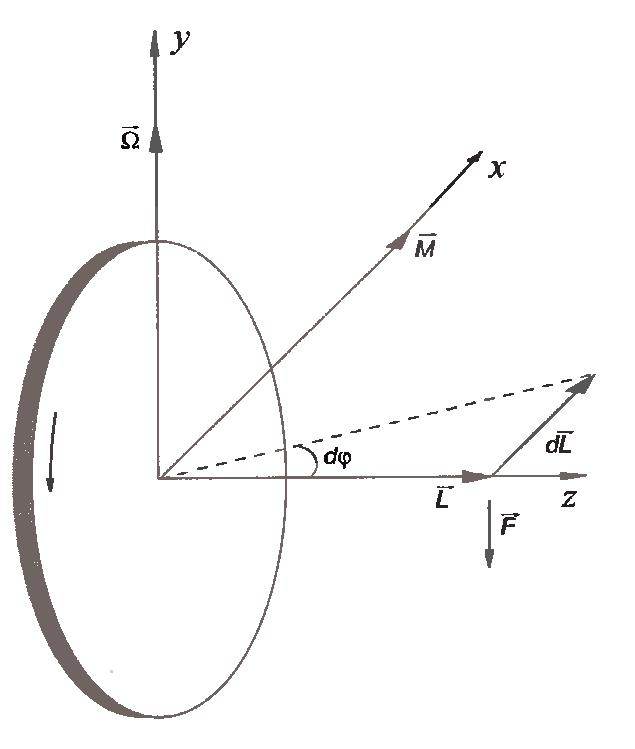
\includegraphics[scale=0.35]{flywheel}
        \end{center}
	\caption{Маховик}
\end{figure}

Под действием момента внешних сил $\vec{M}$ ось гироскопа медленно вращается вокруг оси \textit{y} (рис. 1) с угловой скоростью $\vec{\Omega}$. Такое движение называют \textit{прецессией гироскопа}.

Для изучения регулярной прецессии уравновешенного гироскопа к его оси подвешивают дополнительные грузы. Это смещает общий центр масс и создает момент сил тяжести, вызывающий прецессию. Скорость прецессии в этом случае может быть найдена по формуле:

\begin{equation}
	\Omega = \frac{mgl}{I_0\omega_{0}},
	\label{eq:teor_equation_omega}
\end{equation} 
где $m$ - масса груза, $l$ - расстояние от центра карданова подвеса до точки крепления груза на оси гироскопа. (рис. 2б)

Для выполнения работы используется гироскоп (рис. 2б), закрепленный в карданном подвесе (рис. 2б).


\begin{figure}[h!]  
	\vspace{-2ex} 
	\centering 
	\subfigure[]{
		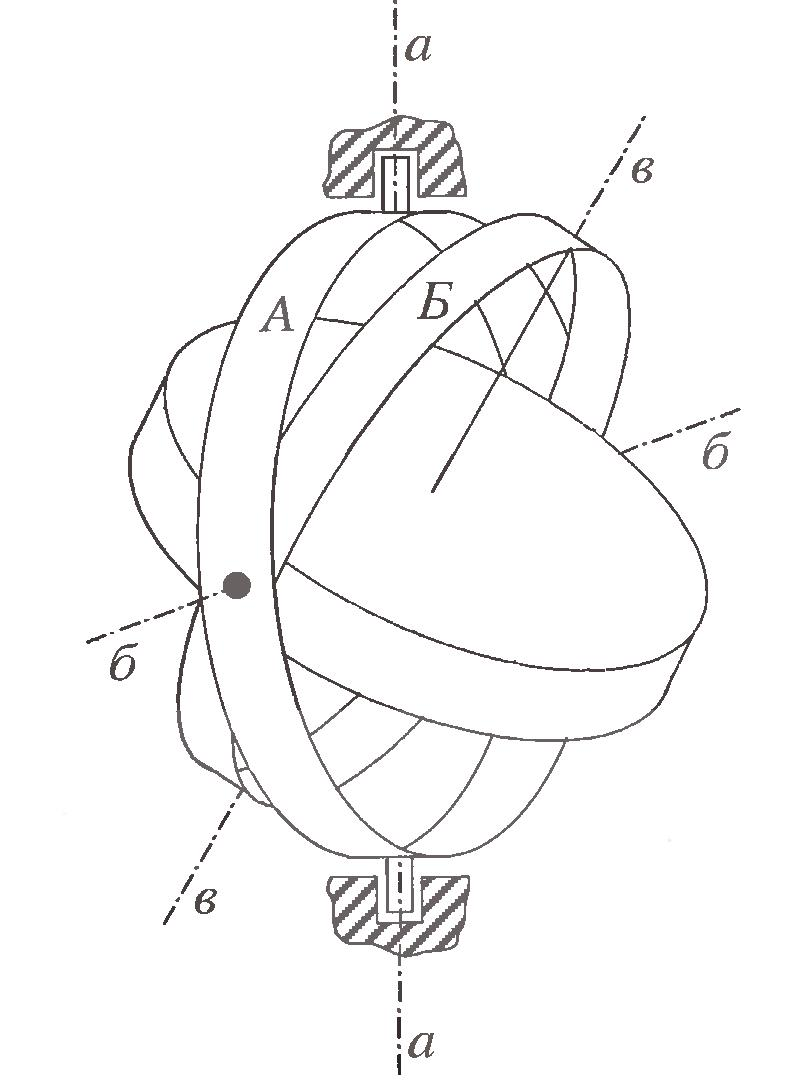
\includegraphics[width=0.29\linewidth]{Cardan_suspension} 	
	\hspace{-2ex}
	\subfigure[]{
		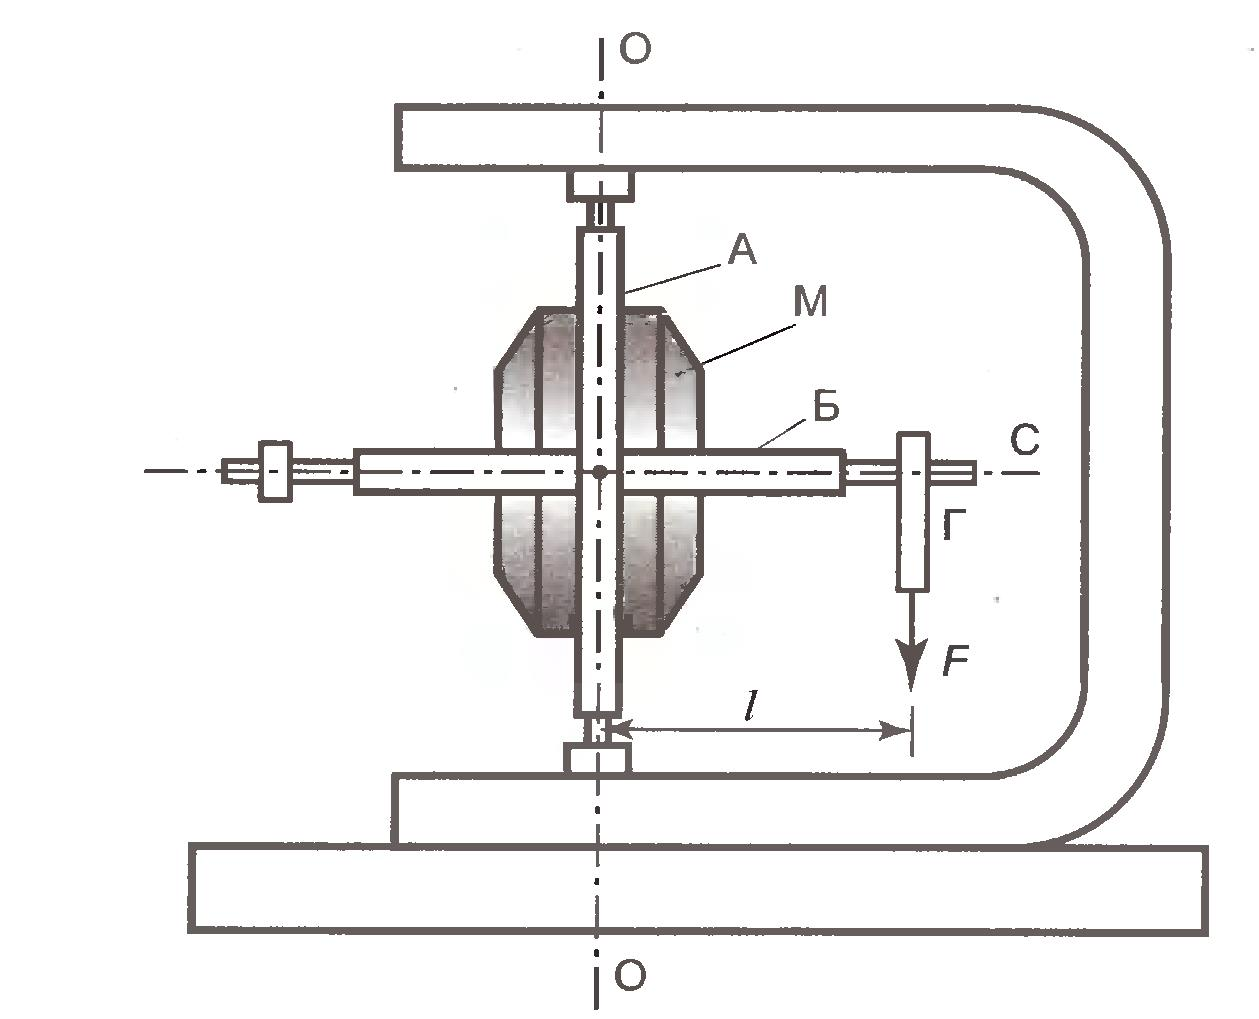
\includegraphics[width=0.45\linewidth]{facility} 
	\caption{а) Гироскоп, закрепленный в карданном подвесе. б) Схема устройства гироскопа.}
\end{figure}

Ротором гироскопа является ротор электромотора М (рис. 2б). Кожух мотора скреплен с кольцом Б (рис. 2а). Мотор с кольцом Б может вращаться в кольце А вокруг горизонтальной оси бб, которое может вращаться относительно оси аа. Рычаг С направлен по оси симметрии ротора. На рычаг подвешивают грузы Г.
%#############################################################################################

%############################################################################################
\section*{Измерения и обработка результатов}

Исследуем зависимость скорости прецессии гироскопа от момента силы, приложенной к его оси. Для этого к оси гироскопа последовательно подвесим грузы различной массы и по количеству оборотов рычага вокруг вериткальной оси и времени, которое на это ушло, опредеим скорость прецесси. Стоит отметить, что в процессе измерений рычаг не только поворачивается в результате прецессси гироскопа, но и опускается из-за моментов сил трения в оси, поэтому в начале опыта приподнимем его на $5-6^\circ$ и закончим опыт, когда рычаг опустится на такой же угол.
Повторим опыт не менее пяти раз для каждого груза. Результаты запишем в табл. 1.

\begin{table}[h!]
	\begin{center}
		\begin{tabular}{|c|c|c|c|c|c|}
			\hline
			\multicolumn{6}{|c|}{$m = 56 \text{ г}\; N = 2$}                                                      \\ \hline
			$t_{\text{полное}}$, c    & 212,33 & 222,26 & 220,32 & 274,96 & 344,9 \\ \hline
			T, c & 35,39 & 44,45 & 55,08 & 68,74 & 86,23 \\ \hline
			\multicolumn{6}{|c|}{$m = 76 \text{ г}\; N = 2$}                                                     \\ \hline	
			$t_{\text{полное}}$, c     & 212,12 & 222,97 & 220,22 & 275,82 & 344,78 \\ \hline
			T, c & 35,35 & 44,59 & 55,06 & 68,96 & 86,00 \\ \hline
			\multicolumn{6}{|c|}{$m = 93 \text{ г}\; N = 2$}                                                    \\ \hline
			$t_{\text{полное}}$, c    & 212,25 & 222,5  & 220,53 & 275,62 & 344,94 \\ \hline
			T, c & 35,38 & 44,50 & 55,13 & 68,91 & 86,24 \\ \hline
			\multicolumn{6}{|c|}{$m =116 \text{ г}\; N = 3$}                                                     \\ \hline
			$t_{\text{полное}}$, c    & 212,09 & 222,56 & 220,31 & 274,79 & 345,03  \\ \hline
			T, c & 35,35 & 44,51 & 55,08 & 68,70 & 86,26 \\ \hline
			\multicolumn{6}{|c|}{$m = 138 \text{ г}\; N = 3$}                                                      \\ \hline
			$t_{\text{полное}}$, c & 212,44 & 222,16 & 220,42 & 275,02 & 345,1 \\ \hline
			T, c & 35,41 & 44,43 & 55,11 & 68,76 & 86,28 \\ \hline
			\multicolumn{6}{|c|}{$m = 174 \text{ г}\; N = 4$} \\ \hline
				$t_{\text{полное}}$, c     & 212,12 & 222,97 & 220,22 & 275,82 & 344,78 \\ \hline
			T, c & 35,35 & 44,59 & 55,06 & 68,96 & 86,00 \\ \hline
			\multicolumn{6}{|c|}{$m = 215 \text{ г}\; N = 4$}                                                    \\ \hline
			$t_{\text{полное}}$, c    & 212,25 & 222,5  & 220,53 & 275,62 & 344,94 \\ \hline
			T, c & 35,38 & 44,50 & 55,13 & 68,91 & 86,24 \\ \hline
			\multicolumn{6}{|c|}{$m = 269 \text{ г}\; N = 4$}                                                     \\ \hline
			$t_{\text{полное}}$, c    & 212,09 & 222,56 & 220,31 & 274,79 & 345,03  \\ \hline
			T, c & 35,35 & 44,51 & 55,08 & 68,70 & 86,26 \\ \hline
			\multicolumn{6}{|c|}{$m = 336 \text{ г}\; N = 5$}                                                      \\ \hline
			$t_{\text{полное}}$, c & 212,44 & 222,16 & 220,42 & 275,02 & 345,1 \\ \hline
			T, c & 35,41 & 44,43 & 55,11 & 68,76 & 86,28 \\ \hline
		\end{tabular}
		\caption{Измерение периодов вынужденной прецессии гироскопа}
		\label{tab:time_and_count_of_rev}
	\end{center}
\end{table}

Усредним периоды прецессии для каждого груза и оценим величину их погрешности.

Систематическая погрешность секундомера равна:
$$\sigma_T^{sist} = 0,01 \text{ с}$$


Случайную погрешность оценим величиной среднеквадратичного отлонения:
$$\sigma_T^{rand} = \sqrt{\frac{1}{N(N - 1)}\sum{(T_i - \langle T \rangle})^2}$$

Полную погрешность найдем как:
$$\sigma_T^{total} = \sqrt{(\sigma_T^{rand})^2 + (\sigma_T^{syst})^2}$$


\begin{table}[h]
	\begin{center}
		\begin{tabular}{|c|c|c|c|c|}
			\hline
			№ груза & $T$ & $\sigma_{\text{сист}}$ & $\sigma_{\text{случ}}$ & $\sigma_{T}$ \\ \hline
			1       & 35,37  & 0,01       & 0,02       & 0,03    \\ \hline
			2       & 44,50  & 0,01       & 0,06       & 0,06    \\ \hline
			3       & 55,09  & 0,01       & 0,03       & 0,03    \\ \hline
			4       & 68,81  & 0,01       & 0,11       & 0,11    \\ \hline
			5       & 86,24  & 0,01       & 0,03       & 0,03    \\ \hline
			6       & 104,84 & 0,01       & 0,08       & 0,08    \\ \hline
			7       & 131,06 & 0,01       & 0,06       & 0,06    \\ \hline
			8       & 159,26 & 0,01       & 0,11       & 0,11    \\ \hline
			9       & 159,26 & 0,01       & 0,11       & 0,11    \\ \hline
		\end{tabular}
		\caption{Период прецессии для различных грузов.}
		\label{tab:periods_and_sigma}
	\end{center}
\end{table}

Перейдем к угловой скорости прецесии:

$$\Omega = \frac{2 \pi}{T}$$

\begin{table}[h!]
	\centering
	\begin{tabular}{|c|c|c|c|c|c|c|c|c|c|}
		\hline
		№ груза & 1      & 2      & 3      & 4      & 5      & 6      & 7      & 8 & 9     \\ \hline
		$\Omega$, рад/c   & 0,0344 & 0,0459 & 0,0568 & 0,0712 & 0,0855 & 0,1074 & 0,1323 & 0,1664 & 0,2083\\ \hline
	\end{tabular}
	\caption{Значения угловой скорости для различных грузов.}
\end{table}

По полученным данным построим график зависимости $\Omega (m)$, убедимся, что она является линейной.

\newpage 

\begin{figure}[h!]
        \vspace{-2ex} 
	\begin{center}
	\includegraphics[scale=0.8]{1.2.5/omega (1).png}
        \end{center}
	\caption{Зависимость угловой скорости прецессии от массы грузов}
\end{figure}

Используя метод наименьших квадратов определим угловой коэффициент прямой $y = kx + b$, наилучшим образом приближающей эксперементальные данные:

$$k = \frac{\langle xy \rangle - \langle x \rangle \langle y \rangle}{\langle x^2 \rangle - \langle x \rangle^2} = 0,620 \text{ рад}/\text{кг} \cdot \text{с}$$
%$$b = \langle y \rangle - k \langle x \rangle$$

Погрешность углового коэффициента:
$$\sigma_k = \frac{1}{\sqrt{n}}\sqrt{\frac{\langle y^2 \rangle - \langle y \rangle^2}{\langle x^2 \rangle - \langle x \rangle^2} - k^2} = 0,001 \text{ рад}/\text{кг} \cdot \text{с}$$

Измерим момент инерции ротора $I_0$ относительно оси симметрии с помощью крутильных колебаний точной его копии, подвешенной вдоль оси симметрии на жёсткой проволоке. Период крутильных колебаний $T_0$ зависит от момента инерции $I_0$ и модуля кручения проволки $f$:

$$T_0 = 2\pi \sqrt{\frac{I_0}{f}}$$

Чтобы исключить модуль кручения проволоки, вместо ротора гироскопа к той же проволоке подвесим цилиндр правильной формы с известными линейными размерами и массой (табл. 4), для которого легко можно вычислить момент инерции $I_c$. Таким образом, для определения момента инерции ротора гироскопа получим:

$$I_0 = I_c\frac{T_0^2}{T_c^2}$$

$$\sigma_{I_0} = I_0\sqrt{(\frac{\sigma_{I_c}}{I_c})^2 + 4(\frac{\sigma_{T_0}}{T_0})^2 + 4(\frac{\sigma_{T_c}}{T_c})^2}$$

Где момент инерции цилиндра может быть найден как:

$$I_c = \frac{md^2}{8}$$

$$\sigma_{I_c} = I_c\sqrt{(\frac{\sigma_m}{m})^2 + 4(\frac{\sigma_d}{d})^2}$$

\begin{table}[h!]
	\begin{center}
		\begin{tabular}{|c|c|c|c|}
			\hline
			 $m$, г& $d$, мм & $I_c$, кг$\cdot$м^2 & $\sigma_{I_c}$, кг$\cdot$м^2 \\ \hline
			 1617,0   & 78,1  &  0,001233 & 0,000003   \\ \hline
		\end{tabular}
		\caption{Параметры цилиндра}
	\end{center}
\end{table}

Период колебаний цилиндра:

\begin{table}[h!]
	\begin{center}
		\begin{tabular}{|c|c|c|c|}
			\hline
			 $N$ & 20 & 20 & 20 \\ \hline
			 $t$, с & 80,2 & 80,1 & 80,2      \\ \hline
              $T_c$, с & 4,010 & 4,005 & 4,010     \\ \hline
              \multicolumn{4}{|c|}{$T_c = 4,008 \pm 0,006 \text{ с}$} \\ \hline
		\end{tabular}
		\caption{Период колебаний цилиндра}
	\end{center}
\end{table}

$$\sigma_{T_c}^{rand} = \sqrt{\frac{1}{n - 1} \sum_{i = 1}^{n} ({T_{ci} - \langle T_c \rangle})^2 } = 0,003 \text{ с}$$

$$\sigma_{T_c}^{syst} = 0,005 \text{ с}$$

$$\sigma_{T_c} = \sqrt{(\sigma_{T_c}^{syst})^2 + (\sigma_{T_c}^{rand})^2 } = 0,006 \text{ с}$$

\newpage

Период колебаний ротора:

\begin{table}[h!]
	\begin{center}
		\begin{tabular}{|c|c|c|c|}
			\hline
			 $N$ & 20 & 20 & 20 \\ \hline
			 $t$, с & 64,1 & 64,2 & 64,2      \\ \hline
              $T_0$, с & 3,205 & 3,210 & 3,210     \\ \hline
            \multicolumn{4}{|c|}{$T_0 = 3,208 \pm 0,006 \text{ с}$} \\ \hline
		\end{tabular}
		\caption{Период колебаний ротора}
	\end{center}
\end{table}

$$\sigma_{T_0}^{rand} = \sqrt{\frac{1}{n - 1} \sum_{i = 1}^{n} ({T_{ci} - \langle T_c \rangle})^2 } = 0,003 \text{ с}$$

$$\sigma_{T_0}^{syst} = 0,005 \text{ с}$$

$$\sigma_{T_0} = \sqrt{(\sigma_{T_0}^{syst})^2 + (\sigma_{T_0}^{rand})^2 } = 0,006 \text{ с}$$

В итоге получим:

$$I_0 = (0,000790 \pm 0,000020) \text{ кг} \cdot \text{м}^2$$

Теперь можем найти частоту вращения ротора:

$$\nu_0 = \frac{\omega_0}{2\pi} = \frac{gl}{2\pi k I_0} = 382,5 \text{ Гц}$$

$$\sigma_{\nu_0} = \nu_0 \sqrt{(\frac{\sigma_k}{k})^2 + (\frac{\sigma_{I_0}}{I_0})^2} = 9,7 \text{ Гц}$$

$$\nu_0 = (382,5 \pm  9,7) \text{ Гц}$$

Скорость вращения ротора гироскопа можно определить и не прибегая к исследованию прецессии. У используемых в работе гироскопов статор имеет две обмотки, необходимые для быстрой раскрутки гироскопа. В данном случае одну обмотку используют для раскрутки гироскопа, а вторую -- для измерения числа оборотов ротора. Ротор электромотора всегда немного намагничен. Вращаясь, он наводит во второй обмотке переменную ЭДС индукции, частота которой равна частоте вращения ротора. Частоту этой ЭДС измеряем по фигурам Лиссажу, получаемым на экране осциллографа, если на один вход подать исследуемую ЭДС, а на другой — переменное напряжение с хорошо прокалиброванного генератора. При совпадении частот на экране получится неподвижный эллипс.\\
При настройке генератора сигнала на частоту $ \nu_0 = 391$ Гц на экране осциллографа виден  неподвижный эллипс, следовательно эта частота сигнала совпадает с частотой вращения ротора гироскопа.

Для оценки момента силы трения, действующего на ось гироскопа, исследуем зависимость опускания оси гироскопа от времени. Результаты проведённых измерений записываем в таблицу

% Please add the following required packages to your document preamble:
% \usepackage{multirow}
\begin{table}[h!]
\centering
\begin{tabular}{|c|c|c|c|c|c|c|}
\hline
№ & $ \Delta \alpha $, рад & $ t $, с & $ \Omega_{f} $, рад/с \\ \hline
1 & 0.17 & 181.60 & 0,00094 \\ \hline%\cline{1-6}
2 & 0.17 & 180.31 & 0,00094 \\ \hline%\cline{1-6}
2 & 0.17 & 183.42 & 0,00093 \\ \hline%\cline{1-6}
2 & 0.17 & 180.98 & 0,00094 \\ \hline%\cline{1-6}
3 & 0.17 & 179.02 & 0,00095 \\ \hline
\multicolumn{4}{|c|}{$\Omega_{f} = 0,00094$ рад/с} \\ \hline
\end{tabular}
\caption{Результат измерения зависимости опускания оси гироскопа от времени}
\label{tab:my-table}
\end{table}

По полученным данным мы можем оценить момент сил, действующих на ось гироскопа по следующей формуле:

\begin{equation}
M_f = \Omega_f I_0\omega_0 = \Omega_f \frac{gl}{k} \approx 0.0018 \text{ Н} \cdot \text{м},
\end{equation}

\section*{Вывод и обсуждение результатов}

В ходе выполнения работы была определена частота вращения ротора гироскопа с помощью исследования прецессионного движения, она составила $\nu_0 = (382,5 \pm  9,7) \text{ Гц}$. Полученная частота в пределах погрешности совпала со значением частоты  $\nu_0 = 391 \text{ Гц}$, измеренной с помощью фигур Лиссажу. Также был оценен момент сил трения, возникающих в оси ротора $M_f \approx 0.0018 \text{ Н} \cdot \text{м}$

В заключение, обратим внимание на предположение $I_{\Omega} \ll I_{\omega_0}$,  с учетом которого теоретические выкладки, привденные в начале работы, справедливы. Учитывая полученные результаты можно заявить, что данное предположение выполняется.
\end{document}
